% \section{Consistency Probing of Knowledge}
\section{Probing PLMs for Consistency}
\label{sec:probe}

In this section, we formally define consistency and describe our framework for probing consistency of PLMs.

% In this section, we formally define consistency and describe our probing framework of PLMs consistency.


\subsection{Consistency}
We define a model as \emph{consistent} if, given  two
\textit{cloze-phrases} such as 
 ``\textit{Seinfeld} originally aired on \textit{[MASK]}'' and
``\textit{Seinfeld} premiered on \textit{[MASK]}'' that
are \textit{quasi-paraphrases}, it makes non-contradictory
predictions\footnote{We refer to \textit{non-contradictory
    predictions} as predictions that, as the name suggest,
  do not contradict one another. For instance, predicting as
  the birth place of a person two difference cities is
  considered to be contradictory, but predicting a city and
  its country, is \textbf{not}.}
%contradicting.}
on N-1 relations over a large set of entities.
A \textit{quasi-paraphrase} -- a concept introduced by \citet{what_is_paraphrase} -- is a more fuzzy version of a paraphrase. The concept does not rely on the strict, logical definition of paraphrase and allows to operationalize concrete uses of paraphrases. This definition is in the spirit of the RTE definition \cite{dagan-rte}, which similarly supports a more flexible use of the notion of entailment.
For instance, a model that predicts \textit{NBC} and \textit{ABC} on the two aforementioned patterns, is not consistent, since these two facts are contradictory. We define a \textit{cloze-pattern} as a cloze-phrase that expresses a relation between a subject and an object.
Note that consistency does not require the answers to be factually correct. While correctness is also an important property for KBs, we view it as a separate objective and measure it independently.
We use the terms \textit{paraphrase} and \textit{quasi-paraphrase} interchangeably.
 


Many-to-many (N-M) relations (e.g. \textit{shares-border-with}) can be consistent 
even with different answers (given they are correct). For
instance, two patterns that express the
\textit{shares-border-with} relation and predict
\textit{Albania} and \textit{Bulgaria} for
%the
\textit{Greece}
%subject
are both correct. We do not consider such relations for measuring consistency. However, another requirement from a KB is \textit{determinism}, i.e., returning the results in the same order (when more than a single result exists).
In this work, we focus on consistency, but also measure determinism of the models we inspect.

\subsection{The Framework}
\label{sec:framework}

\begin{figure*}[t!]
\centering

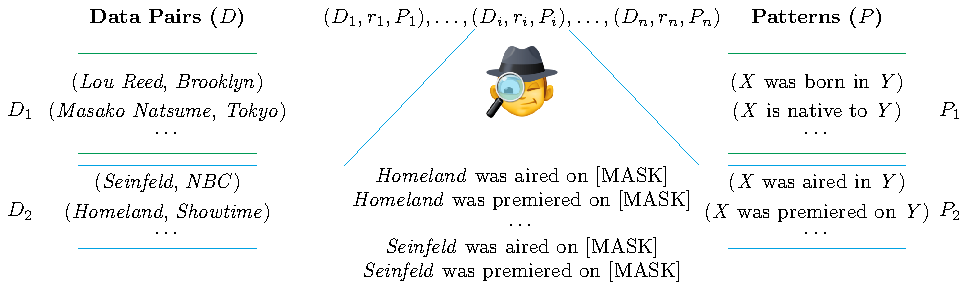
\includegraphics[width=1.\textwidth]{figures/framework}

\caption{Overview of our framework for assessing model
  consistency. $D_i$ (``Data Pairs $(D)$'' on the left) is a
  set of KB triplets of some relation $r_i$, which are
  coupled with a set of \textit{quasi-paraphrase}
  cloze-patterns $P_i$
(``Patterns $(P)$'' on the right)
  that describe that relation. We then populate the subjects
  from $D_i$ as well as a mask token into all patterns $P_i$
(shown in the middle)
  and expect a model to predict the same object across all pattern pairs.}
\label{fig:framework}
% \vspace{-6mm}
\end{figure*}


% \enote{hs}{``quasi-paraphrase cloze-pattern'': it would be
%   better to define clear terminology in the beginning and
%   then to use it consistently (!). it's confusing to the
%   reader to switch back and forth between terms for the same concept}


An illustration of the framework is presented in Figure \ref{fig:framework}.
Let $D_i$ be a set of subject-object KB tuples (e.g., <\textit{Homeland}, \textit{Showtime}>) from some relation $r_i$ (e.g., \textit{originally-aired-on}), accompanied with a set of \textit{quasi-paraphrases} cloze-patterns $P_i$ (e.g., \textit{X} originally aired on \textit{Y}).
Our goal is to test whether the model consistently predicts the same object (e.g., \textit{Showtime}) for a particular subject (e.g., \textit{Homeland}).\footnote{Although it is possible to also predict the subject from the object, in the cases of N-1 relations more than a single answer would be possible, making it impossible to test for consistency, but determinism.} To this end, we substitute \textit{X} with a subject from $D_i$ and \textit{Y} with \textit{[MASK]} in all of the patterns $P_i$ of that relation (e.g., \textit{Homeland} originally aired on \textit{[MASK]} and \textit{Homeland} premiered on \textit{[MASK]}).
A consistent model must predict the same entity. 


% \paragraph{Previous Description}
% Let $D = \{D_1, D_2, \dots, D_m\}$ be a set of sets of KB tuples, where each $D_i$ contains factual statements that express a specific relation $R_i$. In this section, we use $R_1$ = ``premiered on'' and $D_1$ as running examples. Each $D_i=\{d_1^i, d_2^i, \dots, d_n^i\}$ is composed of $n$ examples  where each $d_j^i = <s_j^i,o_j^i>$ is a subject-object tuple from the relation $R_i$. For example, $<\text{\textit{Homeland}}, \text{\textit{Showtime}}>$ is an example of a tuple in $D_1$. Each relation $R_i$ is associated with a set of cloze-patterns $P_i$ that are \textit{quasi-paraphrases} of each other, i.e., they express the same relation $R_i$. For example, $P_1=\{p_1^1, p_2^1, \dots, p_n^1\}$ contains the patterns ``\subj{} was originally aired on \obj{}'' and ``\subj{} premiered on \obj{}''. 


% Given some relation $R_i$, a subject-object tuple $d_j^i \in D_i$ (e.g., `Homeland', `Showtime') and two paraphrases $p_k^i, p_l^i \in P_i$ associated with this relation (such as ``\subj{} was originally aired on \obj{}'' and ``\subj{} premiered on \obj{}''), our goal is to test whether the model consistently predicts the same object for a particular subject. To this end, we substitute \subj{} with a selected subject and \obj{} with MASK; we write this as $p_k^i(s_j^i,mask)$, $p_l^i(s_j^i,mask)$ or (for a specific example) as ``Homeland was originally aired on [MASK]'', ``Homeland was premiered on [MASK]''. Finally, we extract the model's most probable prediction for MASK in the two sentences.  A consistent model must predict the same entity. Note that the consistency measure does not require the answers to be factually correct. While correctness is also an important property for KBs, we view it as a separate objective and measure it independently. 









\paragraph{Restricted Candidate Sets}

Since PLMs were not trained for serving as KBs, they often predict words that are not KB entities; e.g., a PLM may predict, for the pattern ``\textit{Showtime} originally aired on \textit{[MASK]}'', the noun `tv' --  which is also a likely substitution for the language modeling objective, but not a valid KB fact completion.
Therefore, following \citep{Xiong2020Pretrained, kassner2021multilingual}, we restrict the PLMs' output vocabulary to the set of possible gold objects for each relation from the underlining KB. For example, in the \textit{born-in} relation, instead of inspecting the entire vocabulary of a model, we only keep objects from the KB, such as \textit{Paris}, \textit{London}, \textit{Tokyo}, etc.

% I don't think we have to give implementation details at
% this point in the paper?
%In practice, we compute the full probability
%distribution and then only consider the subset of possible
%gold objects.

Note that this setup makes the task easier for the PLM,
especially in the context of KBs. However, poor
consistency in this setup strongly implies that consistency
would be even lower without restricting candidates.
